%----------------------------------------------------------------------------
\chapter{Jegyzőkönyv}
%----------------------------------------------------------------------------
%----------------------------------------------------------------------------
\section{A labor témája}
%----------------------------------------------------------------------------
Egy sáv detektáló szoftver részeit kellett megvalósítani, mely egy videót dolgoz fel. 
Python nyelven, PyCharm fejlesztőkörnyezetet használtunk a mérés során, képfeldolgozó funkciókhoz az OpenCV-t használtuk. 
A fájl betöltő, megjelenítő és szemléltető funkciók már adottak voltak, ezt kellett bizonyos függvényekkel kiegészítenünk, ennek részleteit a következő fejezetek tartalmazzák.

%----------------------------------------------------------------------------
\section{Első feladat}
%----------------------------------------------------------------------------
Az első feladat során a videó egy képe alapján határoztuk meg a sávok pixeleit egy bináris maszkon. 
Ehhez többféle képfeldolgozó eljárást használtunk, melyek együttesen határozták meg a kimenetet.

\begin{figure}[!ht]
	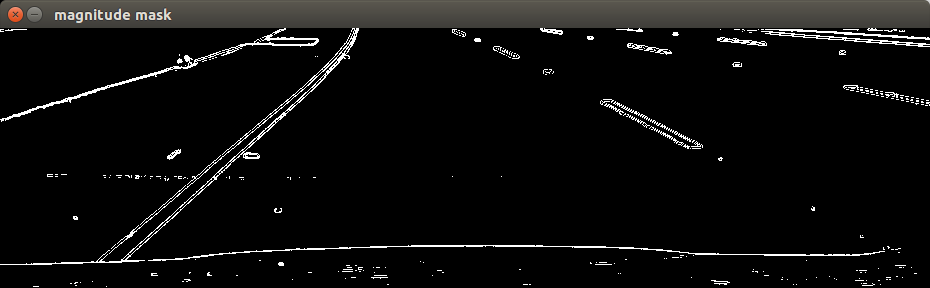
\includegraphics[width=150mm,keepaspectratio]{figures/m09/mag-mask.png}\vspace{2mm}
	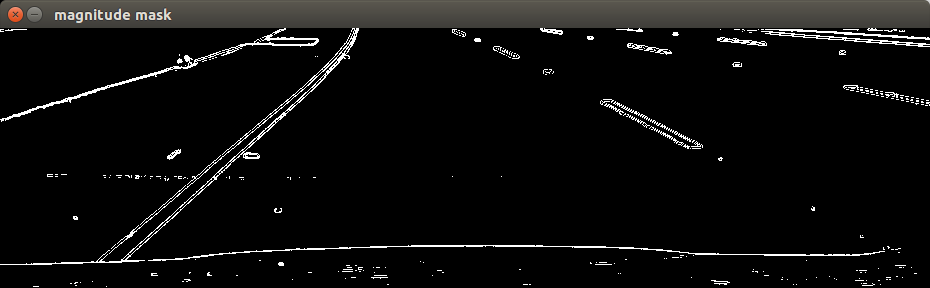
\includegraphics[width=150mm,keepaspectratio]{figures/m09/mag-mask.png}
	\caption{A gradiens abszolút értéke és iránya alapján készített maszk}
	\label{fig:MagDirMask}
\end{figure}

Először a kép pixeleinek x és y irányú gradienseit határoztuk meg Sobel szűrőablakok segítségével. 
Ezt az eredeti kép szürkeárnyalatossá konvertált másolatán tudtuk elvégezni. 
A sávok határait kereshetjük meg a gradiensek segítségével, mivel a fehér sáv és közel fekete úttest pixelei között nagy az intenzitásbeli különbség. 
A kapott értékeket kétféleképpen tettük elérhetővé a kód többi része számára:
\begin{itemize}
	\item Gradiens abszolút értéke: mivel a sávok mindkét határára szükségünk van, nem kell különbséget tennünk a világos-sötét és sötét-világos átmenet között. A szimmetria kiküszöbölésével továbbá elég egy küszöbözés műveletet elvégezni a gradiensekre, nem kell külön negatív és pozitív tartománnyal foglalkozni
	\item Gradiens skálázott értéke: egységes, 0-255 közötti tartományba kényszerítjük külön az x és y irányú gradienseket, ahol a maximális x vagy y irányú gradiens jelenti a 255 értéket. Ezzel nagyság szerint küszöbözhetővé tesszük őket, hiszen például alacsony megvilágítás mellett minden pixel intenzitása kicsi lesz, különbségeik is kicsik maradnak, egy fényes képhez használt küszöbértékek alapján nem találnánk elég nagy intenzitás eltéréseket.
\end{itemize}
Intenzitás alapú szűrést a skálázott gradiensek összegére végeztük el, míg az irány szerinti szűréshez a két irány arkusztangensére, a keresett értéktartományok adottak voltak. Az így készített maszk látható a \figref{MagDirMask}~ábrán.


Másodszor szín szerinti szűrést alkalmaztunk, ehhez HLS színtérbe konvertáltuk a képet. Mivel csak fehér színt kerestünk, elég volt a színtér S, azaz telítettség értékére szűrni, ez fehér közeli színekre nagy értékű lesz, ezt a \figref{ColorMask}~ábra mutatja.

\begin{figure}[!ht]
	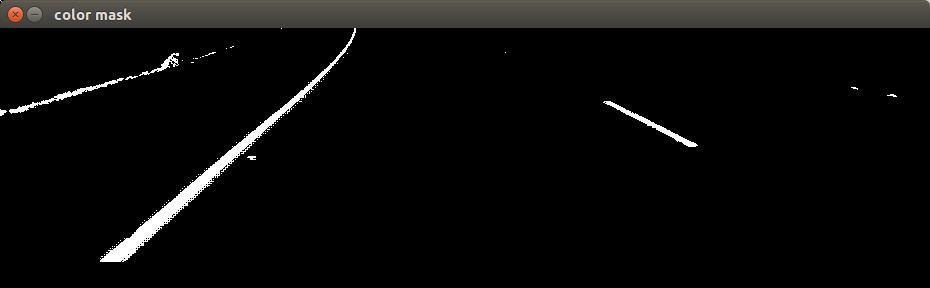
\includegraphics[width=150mm,keepaspectratio]{figures/m09/color-mask.png}
	\caption{A színszűrés alapján készített maszk}
	\label{fig:ColorMask}
\end{figure}

Végül sávnak nyilvánítottunk minden nagy és megfelelő irányú gradiensvektor által jelölt vagy megfelelő színű pixelt. Ezzel a két módszer hibáit szűrtük ki: a gradiens módszer a sáv széleit, míg a szín módszer a belsejét találja meg, a kettő uniója jelenti a teljes sávot, ez látható a \figref{CombinedMask}~ábrán.

\begin{figure}[!ht]
	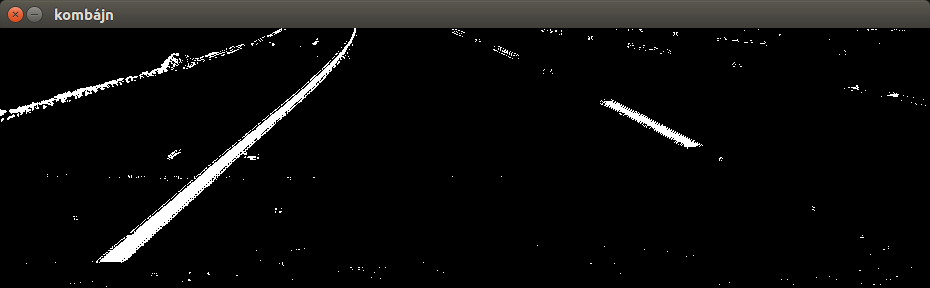
\includegraphics[width=150mm,keepaspectratio]{figures/m09/combined-mask.png}
	\caption{A kombinált maszk}
	\label{fig:CombinedMask}
\end{figure}
\newpage

%----------------------------------------------------------------------------
\section{Második feladat}
%----------------------------------------------------------------------------
Egy konstans paraméterű perspektív transzformációt hajtottunk végre az első feladatban elkészített maszkon. Ehhez négy pontot kellett megadni a síkon, majd ezek transzformáció utáni megfelelőit, az átalakítást mátrixát az OpenCV \textit{getPerspectiveTransform} függvénye számolta ki, a transzformációt pedig a \textit{warpPerspective} függvény végezte el a mátrix alapján. Ennek eredménye a \figref{Warped}~ábrán látható. Az átalakítás inverzét is el kellett tárolnunk, hogy a torzított képen meghatározott sávok helyét megkaphassuk az eredeti képen is.

\begin{figure}[!ht]
	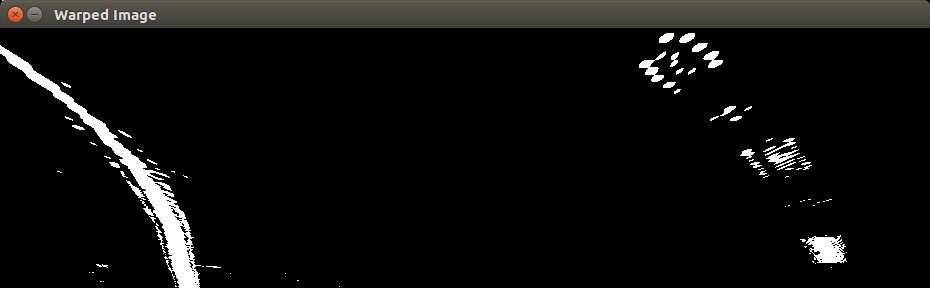
\includegraphics[width=150mm,keepaspectratio]{figures/m09/warped-mask.png}
	\caption{A transzformált maszk}
	\label{fig:Warped}
\end{figure}

Egy hisztogramot készítettünk, mely a \figref{Histogram}~ábrán látható. Ez a torzított kép fehér pixeleinek számát tartalmazta oszloponként összesítve. Mivel az egyenes sávok egyenes oszlopokként jelennek meg ezen a képen, ott helyezkedik el a sáv, ahol az oszlopban sok a sávnak címkézett pixel. A hisztogram két lokális maximuma jelenti a két sávot. Ha az egyik maximum jóval kevesebb, mint a másik, az szaggatott felfestésre utal. A sávok görbülhetnek is, ekkor a felső részük már nem esik a sáv aljának oszlopába. Ezért csak a torzított maszk alsó felét vesszük figyelembe a hisztogram készítésekor, azon a részen a sáv görbülettől függetlenül megközelítőleg oszlopként látszik.


\begin{figure}[!ht]
	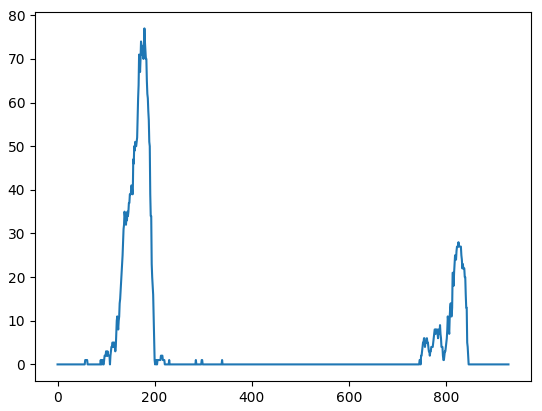
\includegraphics[width=150mm,keepaspectratio]{figures/m09/histogram.png}
	\caption{A vertikális hisztogram}
	\label{fig:Histogram}
\end{figure}
\newpage

%----------------------------------------------------------------------------
\section{Harmadik feladat}
%----------------------------------------------------------------------------
A kamera és a detektálás is zajos eredményeket produkál, a jármű irányításához azonban célszerű ezt kiszűrni, simább bemenetet szolgáltatni. A program előre megírt részei kiszámolták a sáv görbületét és a jármű sávközéptől való eltérését, ezeket dolgoztuk fel. 

Az új értékeket egy-egy tömbben tároljuk, a tömb elemeinek átlaga adja a simított értéket. Mozgó átlagot számolunk, azaz a tömb teljes feltöltése után a legrégebbi értéket eldobtuk, az újat beszúrtuk, majd átlagot számoltunk az elemekből.
A simított eltérés értékekre LS becsléssel egyenest illesztettünk, az egyenes egyenlet alakját egy mátrix definiálta. Az egyenes becsült meredeksége jelenti majd a szabályzó számára a középtől való eltérés változását.


\newpage
%----------------------------------------------------------------------------
\section{Negyedik feladat}
%----------------------------------------------------------------------------
A fuzzy szabályzót a klasszikus MacVicar-Wheelan metaszabályok szerint terveztük meg. Bemenetnek a hibajelet, illetve annak deriváltját adtuk, melyekhez 5-5 tagsági függvényt alkottunk. A kimenet szintén 5 tagsági függvénnyel rendelkezik. Ezek alapján 5 fuzzy szabályt hoztunk létre.

\begin{figure}[!ht]
	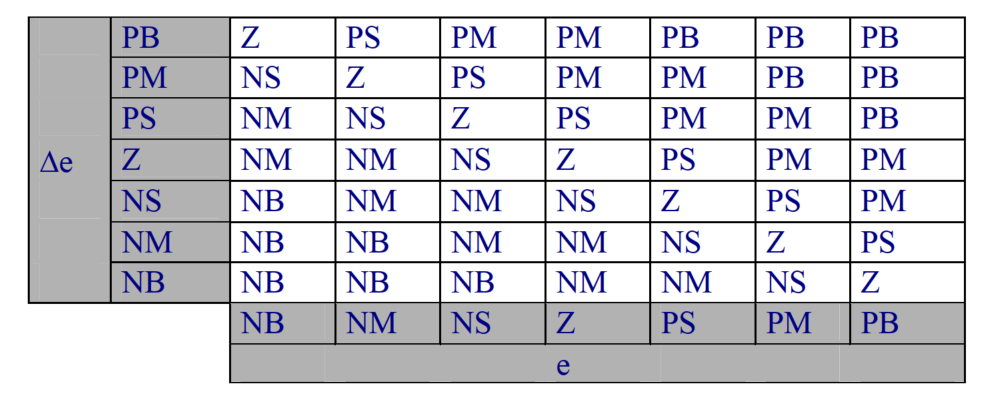
\includegraphics[width=150mm,keepaspectratio]{figures/m09/mcw.png}
	\caption{Példa a MacVicar-Wheelan metaszabályokra, 7-7 be-, és kimeneti tagsági függvények alapján}
	\label{fig:MCW}
\end{figure}


%----------------------------------------------------------------------------
\section{Ötödik feladat}
%----------------------------------------------------------------------------
A kész programot futtatva az általunk implementált detektáló és szabályzó algoritmus eredményét előre megírt függvények szemléltették a videón. A sávok közötti terület színes jelölése pontosan követte a felfestés közötti területet, a horizont környékén vált bizonytalanná a becslés, főleg kanyarodás közben, hajlamos volt a színes terület eltérni a valóságtól. 

Az úthibák hatására az autó belengése miatt a kamera és az út síkja változik, emiatt a megadott négy pont a perspektív transzformáció során helytelenné vált, ilyen esetekben is pontatlanná vált a becslés.

Egy grafikonon (\figref{Results}~ábra) láthattuk a szabályzó bemeneteit és kimenetét, az értékek csillapított és nyers formáját is. A zaj nagyrészt valóban eltűnt a simítás után.



\begin{figure}[!ht]
	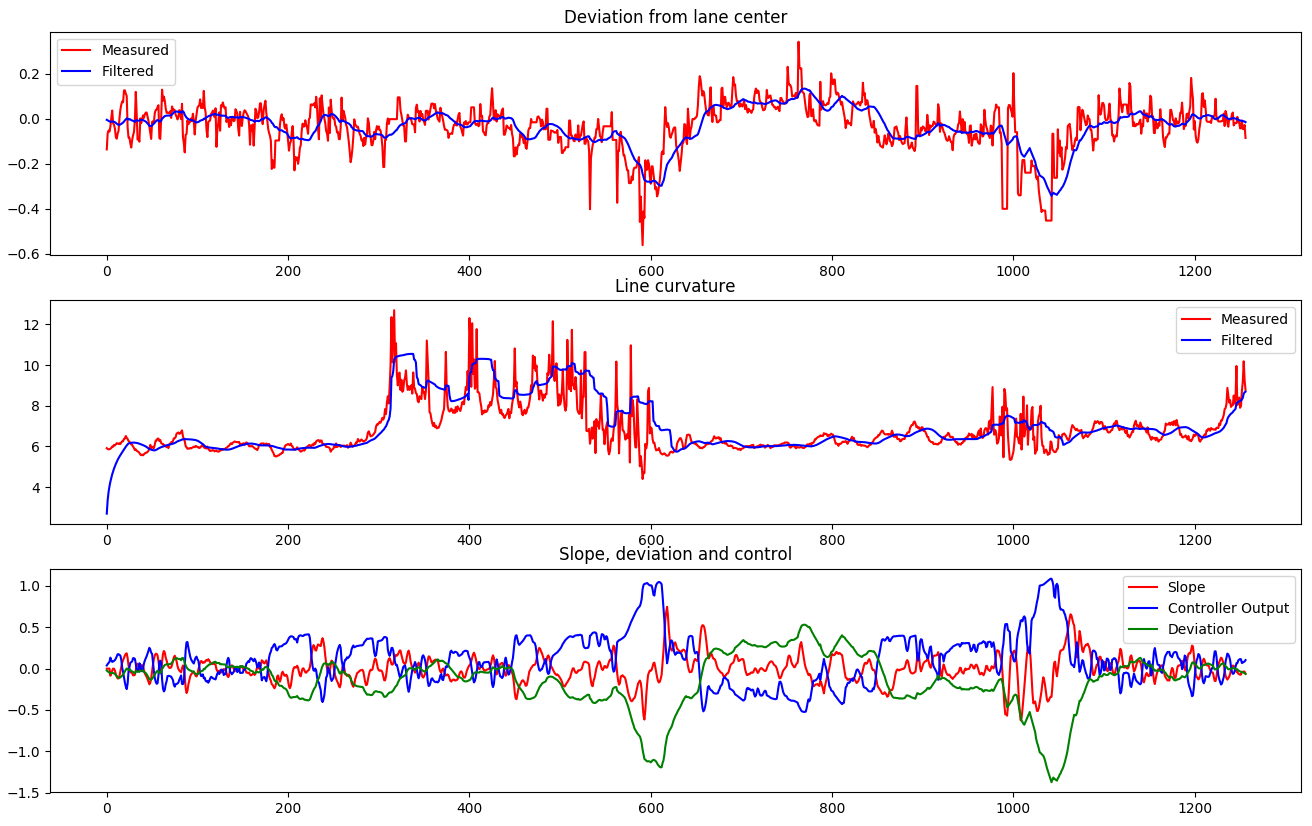
\includegraphics[width=150mm,keepaspectratio]{figures/m09/results.png}
	\caption{Az algoritmus működésének ellenőrzése}
	\label{fig:Results}
\end{figure}







